%This is a LaTeX template for homework assignments
\documentclass{article}
\usepackage[utf8]{inputenc}
\usepackage{amsmath}
\usepackage[russian]{babel}
\usepackage{xcolor}
\usepackage{hyperref}
\definecolor{linkcolor}{HTML}{799B03} % цвет ссылок
\definecolor{urlcolor}{HTML}{799B03} % цвет гиперссылок
\usepackage{graphicx}

\hypersetup{pdfstartview=FitH,  linkcolor=linkcolor,urlcolor=urlcolor, colorlinks=true}

\begin{document}

\section*{Задача A} 

\subsection*{Условие} 
Найти значения переменных в формуле 3SAT, при которых наибольшее число
скобок принимают истинное значение.
\subsection*{Доказательство NP}
Допустим, что всего $n$ переменных и $m$ скобок.
\begin{enumerate}
\item Переформулируем задачу

Можно ли подобрать такие значения переменных, чтобы истинно было хотя бы $K$ скобок?

\item Сертификат: последовательность $(k, x_1, x_2, ..., x_n)$
\item Верификатор: Посчитать количество истинных скобок. Сравнить с k.

\end{enumerate}
\subsection*{Доказательство NPH}
Надо доказать, что $3SAT \leq_p MAX3SAT$. Допустим, что $MAX3SAT <_p 3SAT$, тогда у нас есть  $(k, x_1, x_2, ..., x_n)$ такое, что $k$ скобок истинны, а значит хотя бы 1 истинна, то есть решена задача $3SAT$, а значит  допущение($MAX3SAT <_p 3SAT$) неверное, то есть получено противоречие. Это значит, что исходное утверждение верно.
\newpage

\section*{Задача G} 

\subsection*{Условие} 
Дана матрица $A$ размера $M \times N$ из целых чисел, вектор $B$ размера $M$ из целых чисел. Найти бинарный вектор $x$, такой что $Ax \leq B$.

\subsection*{Доказательство NP}
\begin{enumerate}
\item Сертификат: Бинарная последовательность чисел размера $M$. Очевидно, что размер сертификата равен $M$, то есть он полиномиален относительно размера самой задачи.
\item Верификатор: Непосредственно производит умножение и поэлементное сравнение. Самый очевидный алгоритм умножения матриц имеет сложность $O(n^3), n = max(M, N)$, сравнение выполняется за $O(M)$. А значит, верификатор работает за полиномиальное время от входа.
\end{enumerate}

\subsection*{Доказательство NPH}


\newpage
\section*{Задача K} 
\subsection*{Условие} 
Дан взвешенный ориентированный граф $G = (V, E)$, найти в нем гамильтонов путь.

\subsection*{Доказательство NP}
Допустим, всего N вершин.
\begin{enumerate}
\item Сертификат: Последовательность вершин размера $N$. Очевидно, что размер сертификата равен N, то есть он полиномиален относительно размера самой задачи.
\item Верификатор: Проверяет, посещены ли все вершины(достаточно проверить, что в сертификате все элементы уникальны) и существуют ли все ребра между соседними элементами в последовательности.
\end{enumerate}

\subsection*{Доказательство NPH}
Для доказательства этого факта сведем задачу о поиске гамильтонова цикла (далее - ГЦ) в ориентированном графе к задаче о поиске гамильнового пути (далее - ГП) в ориентированном графе.

Пусть дан граф. Выберем произвольную вершину графа $d$ и раздвоим ее на $d1$ и $d2$, так, что все входящие дуги в $d$ теперь будут входить в $d2$, а все исходящие дуги из $d$ теперь будут выходить из $d1$. \\

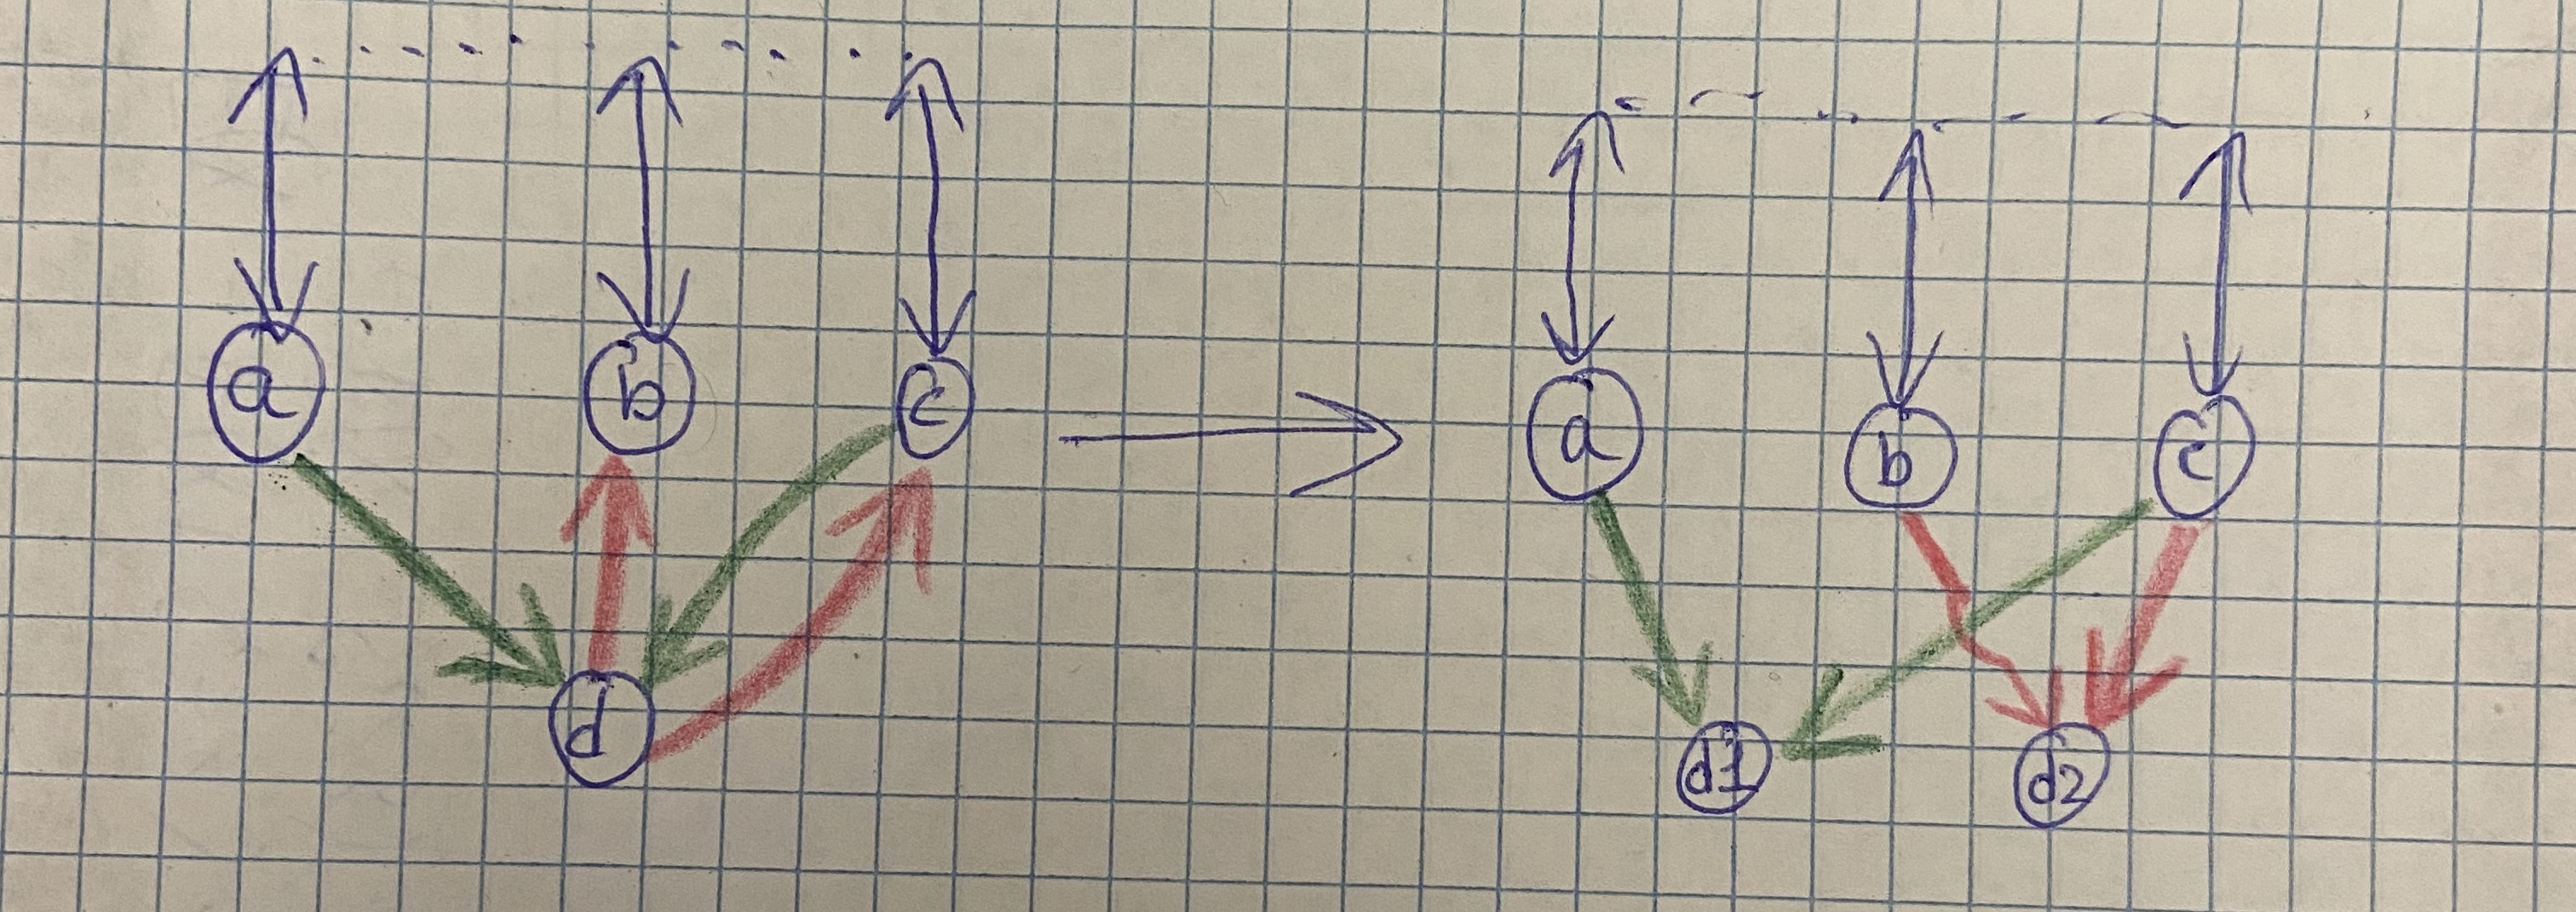
\includegraphics[totalheight=4cm]{IMG_0864.jpg}

\begin{enumerate}
\item В одну сторону.

Утверждается, что если в исходном графе был ориентированный ГЦ, то в полученном будет ориентированный ГП. Докажем это утверждение. Допустим, что в исходном графе был ГЦ. Без ограничения общности будем считать, что он начинался и заканчивался в вершине $d$. Тогда после такого преобразования будет существовать ГП и он будет начинаться в $d2$ и заканчиваться в $d1$.

\item В обратную сторону.

Если в полученном графе будет ГП, то есть будет путь соединяющий все вершины, тогда он будет посещать вершины $d1$ и $d2$. Это значит, что он будет начинаться в $d2$ и заканчиваться в $d1$. Таким образом, если объединить эти вершины, то в полученном графе будет существовать ГЦ.


\end{enumerate}

Использована информация из: \href{https://neerc.ifmo.ru/wiki/index.php?title=NP-полнота_задач_о_гамильтоновом_цикле_и_пути_в_графах}{Ссылка на источник} .

\newpage

\section*{Задача O} 

\subsection*{Условие} 
Дан набор задач $A$, для каждой есть время, за которое ее решает один процессор  $t_i$, $M$ процессоров и общий дедлайн $D$. Можно ли разбить все задачи на непересекающиеся множества задач $A_j$, такие что $\bigcup_{j=1}^{n} A_j = A$ и сумма $t_i$ по каждому $A_j \leq D$. Формально: $\forall j\ \sum_{i \in A_j} t_i \leq D$

\subsection*{Доказательство NP}
Допустим, что всего задач $N$.
\begin{enumerate}
\item Сертификат: последовательность $k_1, k_2, ..., k_N: \forall i\ k_i \in \{1, 2, ..., M\}$
\item Верификатор: Перебирает все процессоры, считает время работы на нем (суммирует те $t_j$, у которых $k_j$ равно номеру этого процессора), если оно больше $D$ хоть в одному случае, то возвращает ЛОЖЬ, иначе ИСТИНУ.
\end{enumerate}

\subsection*{Доказательство NPH}
Сведем задачу о рюкзаке к этой задаче. В задаче о рюкзаке у каждого объекта есть вес $w_j$ и стоимость $c_j$ . В нашей задаче $w_j = c_j = t_j$. Тогда 

\newpage
\section*{Задача  R} 

\subsection*{Условие} 
Рассмотрим такой алгоритм построения максимальной клики: будем каждый раз
удалять из графа вершину минимальной степени, пока не получим полный граф.
Докажите или опровергните, что такой алгоритм дает решение, не более чем в X
раз отличающееся от оптимального.

\subsection*{Решение} 
\textbf{Утверждение.} Если клика размера $N$, то все входящие в нее вершины имеет степень $= N - 1$. Доказательство очевидно.
\\
\hfill \\
\textbf{Утверждение.} Для любого $n$ можно построить граф, в котором степень хотя бы одной вершины будет $n$, а всех остальных вершин будет $\geq n$, а размер максимальной клики будет 2. \\
\#
Этот факт требует доказательства, но у меня не получилось это доказать (и найти доказательство тоже не получилось). Я построил для размера 2 и для размера 3. Кажется, что это утверждение истинно и доказать его можно.
\#
\\
\hfill \\
\textbf{Утверждение.} Для любого $N$, существует граф, в котором есть клика размера $N$ и используя этот алгоритм будет получаться клика размера 2. 
\#
Возьмем клику $C$ размера $N + 1$. Возьмем граф $G$, в котором существует вершина $v$, степень которой $N$, а степень всех остальных вершин $\geq N$. Соединим $C$ и $G$ любым ребром, главное, чтобы оно не касалось вершины $v$. В получившемся графе минимальная степень вершины $N$ и существует вершина степени $N$, входившая в граф $C$. Допустим алгоритм начнет удаление именно с этой вершины. Затем он будет постоянно удалять все вершины графа $C$, так как при удалении вершины графа $C$, степень всех вершин графа $C$ уменьшиться на 1. Таким образом граф $C$ будет полностью удален и задача сведется к нахождению максимальной клики в графе $G$. А у этого графа максимальная клика имеет размер 2 по определению.
\#

\subsection*{Вывод} Последнее утверждение опровергает существование константы $X$.



\end{document}








